\section{Introduction}

Neural networks have been widely used in various machine learning applications, achieving comparable or better performance than existing methods without requiring highly engineered features \citep{krizhevsky2012imagenet}. However, neural networks have several intriguing aspects that defy conventional views of statistical learning theory and optimization, thereby hindering the architecture design and interpretation of these models. For example, despite having more parameters than training examples, deep neural networks generalize well without an explicit form of regularization \citep{zhang2016understanding,neyshabur2017geometry,arora2019implicit}. \cite{zhang2016understanding} also observe that neural networks can perfectly fit corrupted labels while maintaining a certain amount of generalization power\footnote{This property also holds for the $1$-nearest neighbors algorithm.}.


		%The on the torus function in (a)-(c). 
		% The Pearson correlation between the relative similarity based on two-layer neural nets and the geodesic distance on the torus function is $-0.97$.
		% We then compare the local elasticity of three-layer neural nets and three-layer linear neural networks on the two folded plane function in (d)-(f). 
		%The Pearson correlation of the relative similarity based on three-layer neural nets and the geodesic distance on the two folded plane functions is $-0.92$. 
		%%We therefore use linear neural networks in simulations and hold over-parameterization constant to prevent it influencing experimental results. The blue points in Figure (a) and (d) denote the primary examples and the red points denote the auxiliary examples. Our simulations are based on the primary examples.}

%%However, the ``black-box'' nature of neural networks makes it difficult to explain the behaviors. For example, why neural nets with stochastic gradient descent (SGD) exhibit strong ability in memorization, generalization, and robustness is still unclear \citep{zhang2016understanding, krueger2017closer,rolnick2017deep}. These mysteries directly hinder the design and the usage of neural nets. Accordingly, there is an explosion of interest in interpreting these black-box models, with the goal of better understanding their behaviors. One direction is to illustrate model predictions. 

%%Researchers have tried to visualize the representations and activation patterns of neural nets, and analyze the correlations between neurons or examples \citep{zhang2018visual, hohman2018visual,raghu2017svcca, sellam1like, li2019beyond, zhang2018interpreting, dumitru2018learning, murdoch2018beyond, koh2017understanding}. 
%However, these visual interpretations and correlation analysis hardly explain the performance of neural networks. Another direction leads to the theoretical analysis of optimization and generalization \citep{ALS2018-dnn, allen2018learning, du2019gradientglobal, du2019gradient, nguyen2017loss}. Theoretical results are yet criticized for being less practical, and the generalization analysis is largely limited to special cases. Recently, researchers defined Neural Tangent Kernel (NTK) to connect kernels and neural nets in the infinite width limit \citep{jacot2018neural, yang2019scaling, arora2019exact, lee2019wide}. However, some subsequent work shows that kernels can not be used to explain the regularization and some special function classes \citep{allen2019can, wei2018margin}. 

%%\subsection{A Persistent Phenomenon}
%\subsection{Our Contributions}

In this paper, we complement this line of findings by proposing a hypothesis that fundamentally distinguishes neural networks from linear classifiers\footnote{Without using the kernel trick, these classifiers include linear regression, logistic regression, support vector machine, and linear neural networks.}. This hypothesis is concerned with the dynamics of training neural networks using stochastic gradient descent (SGD). Indeed, the motivation is to address the following question:
\begin{center}
{\centering \it How does the update of weights using SGD at an input $\bx$ and its label $y$ \\impact the prediction of the neural networks at another input $\bx'$ ?} 
\end{center}
%%\hangfeng{We only consider the $\bx'$ with the same label as $\bx$ in our experiments.} \weijie{we will make this explicit later.}
Taking this dynamic perspective, we make the following three contributions.

%\begin{itemize}
%    \item 

First, we hypothesize that neural networks are \textit{locally elastic} in the following sense: an extensive set of experiments on synthetic examples demonstrate that the impact on the prediction of $\bx'$ is significant if $\bx'$ is in a \textit{local} vicinity of $\bx$ and the impact diminishes as $\bx'$ becomes far from $\bx$ in an \textit{elastic} manner. In contrast, local elasticity is not observed in linear classifiers due to the leverage effect \citep{weisberg2005applied}. Thus, at a high level, local elasticity must be inherently related to the nonlinearity of neural networks and SGD used in updating the weights. This phenomenon is illustrated by Figure~\ref{fig:simulations}. Additional synthetic examples and ImageNet \citep{deng2009imagenet} with a pre-trained ResNet \citep{he2016deep} in Appendix \ref{subsec:more-simulations} further confirm local elasticity. For completeness, we remark that the notion of local elasticity seems related to influence functions on the surface
\citep{koh2017understanding}. The fundamental distinction, however, is that the former takes into account the dynamics of the training process whereas the latter does not. See Section~\ref{sec:def} for a formal introduction of the notion of local elasticity.

\begin{figure*}[t]
        %\begin{minipage}{0.35\textwidth}
		\centering
		 	\subfigure[The torus.]{
			\centering
			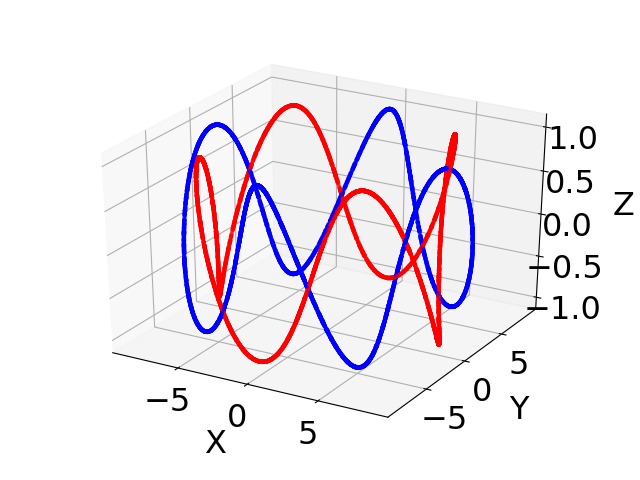
\includegraphics[scale=0.29]{Figures/donut.png}
			\label{fig:torus}}
        %\hspace{0.01in}
        	\subfigure[Two-layer nets fitting the torus.]{
			\centering
			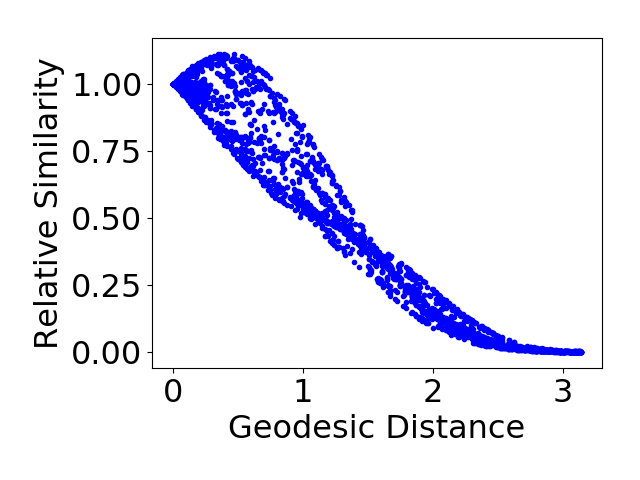
\includegraphics[scale=0.26]{Figures/donut_MLPNet_ripple_optimal.png}
			\label{fig:torus-NNs}}
        %\hspace{0.01in}
     	\subfigure[Two-layer \textit{linear} nets fitting the torus.]{
			\centering
			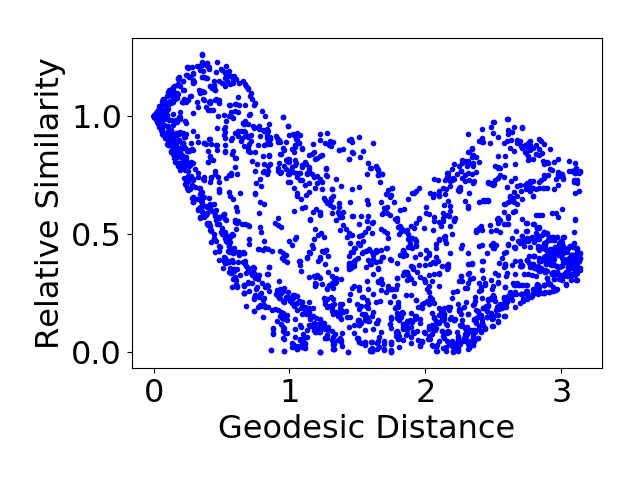
\includegraphics[scale=0.26]{Figures/donut_MLPLinear_ripple_optimal.png}
			\label{fig:torus-linear}}\\[-2ex]
        %\hspace{0.01in}
        %\end{minipage}
        %\begin{minipage}{0.35\textwidth}
		    \subfigure[The two folded boxes.]{
			\centering
			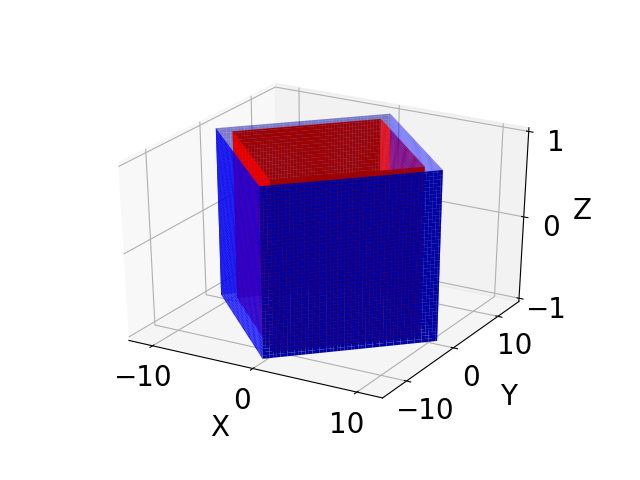
\includegraphics[scale=0.29]{Figures/two_fold_surface-fine.png}
			\label{fig:two-fold-surface}}
        %\hspace{0.01in}
        	\subfigure[Three-layer nets fitting the boxes.]{
			\centering
			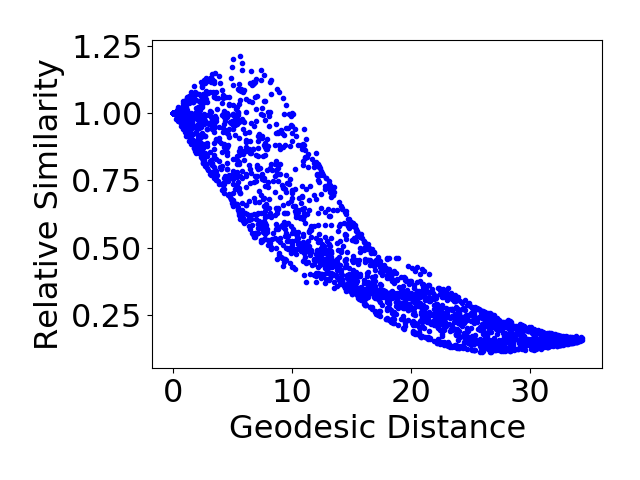
\includegraphics[scale=0.26]{Figures/two_fold_surface_MLPNet3Layer_ripple_optimal.png}
			\label{fig:two-fold-surface-NNs}}
        %\hspace{0.01in}
     	\subfigure[Three-layer \textit{linear} nets fitting the boxes.]{
			\centering
			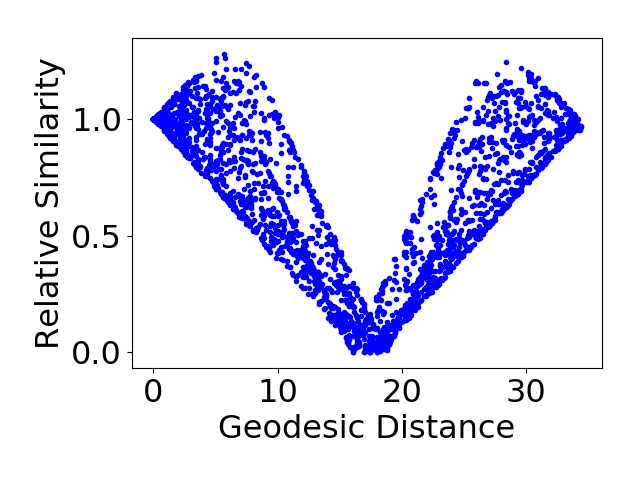
\includegraphics[scale=0.26]{Figures/two_fold_surface_MLPLinear3Layer_ripple_optimal.png}
			\label{fig:two-fold-surface-linear}}
		\caption{Comparisons between ReLU neural networks and linear neural networks in terms of local elasticity. In the left column, the red points form one class and the blue points form the other class. The linear nets are of the same sizes as their non-linear counterparts. The details on how to construct the torus and boxes can be found in Appendix \ref{subsec:functions} and the network architectures are described in Appendix~\ref{sec:disc-some-terms}. During the training process of the neural networks, we plot the geodesic distance (see more details in Appendix \ref{subsec:functions}) between two blue points $\bx$ and $\bx'$, and their relative prediction changes (see its definition in Equation (\ref{eq:sr})) in (b), (c), (e), and (f). The correlations of (b), (c), (e), and (f) are $-0.97$, $-0.48$, $-0.92$, and $-0.14$, respectively. (b) and (e) show that the distance and the relative change exhibit decreasing monotonic relationship, thereby confirming local elasticity, while no monotonic relationship is found in (c) and (f). }		
\label{fig:simulations}
\end{figure*}

Furthermore, we devise a clustering algorithm by leveraging local elasticity of neural networks. In short, this algorithm records the relative change of the prediction on a feature vector to construct a similarity matrix of the training examples. Next, the similarity matrix is used by, for example, $K$-means to partition the points into different clusters. The experiments on MNIST \citep{lecun1998mnist} and CIFAR-10 \citep{krizhevsky2009learning} demonstrate the effectiveness of this local elasticity-based clustering algorithm. For two superclasses (e.g., mammal and vehicle), the algorithm is capable of partitioning the mammal class into cat and dog, and the second superclass into car and truck. These empirical results, in turn, corroborate our hypothesis that neural networks (with
nonlinear activation) are locally elastic. The code is publicly available at \url{https://github.com/hornhehhf/localelasticity}. See the description of the algorithm in Section~\ref{sec:local-elast-based} and experimental results in Section~\ref{sec:experiments}.


Finally, this paper provides profound implications of local elasticity on memorization and generalization of neural networks, among others.  In this spirit, this work seeks to shed light on some intriguing aspects of neural networks. Intuitively, the locality part of this property suggests that the neural networks can efficiently fit the label of an input without significantly affecting most examples that have been well fitted. This property is akin to the nearest neighbors algorithm (see, e.g., \citet{papernot2018deep}). Meanwhile, the elasticity part implies that the prediction surface is likely to remain smooth in the training process, in effect regularizing the complexity of the nets in a certain sense. These implications are discussed in detail in Section~\ref{sec:conclusion}.


\subsection{Related Work}

There has been a line of work probing the geometric properties of the decision boundary of neural networks. \cite{montufar2014number} investigate the connection between the number of linear regions and the depth of a ReLU network and argue that a certain intrinsic rigidity of the linear regions may improve the generalization. \cite{fawzi2017classification,fawzi2018empirical} observe that the learned decision boundary is flat along most directions for natural images. See \cite{hanin2019complexity} for the latest development along this line and \cite{fort2019stiffness} for a dynamic perspective on the landscape geometry.

%%makes the observation that \weijie{in the vicinity of natural images, the decision boundaries learned by deep networks are flat along
%most (but not all) directions, and that some curved directions are shared across datapoints.}
%%There has been prior work explaining the unreasonable effectiveness of neural nets. We briefly review recent work about interpreting neural nets. 

In another related direction, much effort has been expended on the expressivity of neural networks, starting from universal
approximation theorems for two-layer networks \citep{cybenko1989approximation,hornik1989multilayer,barron1993universal}. Lately, deep neural networks have been shown to possess better representational power than their shallow counterparts \citep{delalleau2011shallow,telgarsky2016benefits,eldan2016power,mhaskar2016deep,yarotsky2017error,chen2019efficient}. From a nonparametric viewpoint, approximation risks are obtained for neural networks under certain smooth assumptions on the regression functions \citep{schmidt2017nonparametric,suzuki2018adaptivity,klusowski2018approximation,liang2018well,bauer2019deep,ma2019barron}.

%%%(Cybenko, 1989; Mhaskar, 1993; Delalleau 
%%Bengio, 2011; Mhaskar  Poggio, 2016; Eldan  Shamir, 2016; Telgarsky, 2016; Cohen  Shashua,
%%2016). All of these results are at the population level characterizing which mathematical functions
%%certain families of neural networks can express over the entire domain. We instead study the representational power of neural networks for a finite sample of size n. This leads to a very simple proof
%that even O(n)-sized two-layer perceptrons have universal finite-sample expressivity. \cite{suzuki2018adaptivity,schmidt2017nonparametric,klusowski2018approximation,bauer2019deep} \cite{klusowski2018approximation, bauer2019deep}

%%%One direction is to illustrate the behaviors of neural nets through the empirical analysis. \cite{zhang2016understanding} demonstrate that neural nets easily fit random labels. \cite{krueger2017closer} show that neural nets learn simple patterns first before memorizing. \cite{rolnick2017deep} neural nets are robust to massive label noise. These works analyze the behaviors of neural nets on memorization, generalization and robustness thorough experiments. \cite{ulyanov2018deep} make use of a property of neural nets that the parametrization offers high impedance to noises and low impedance to signals to provide a handcrafted image prior for standard inverse problems such as denoising, super-resolution, and inpainting.

A less related but more copious line of work focuses on optimization for training neural networks. A popular approach to tackling this problem is to study the optimization landscape of neural networks \citep{choromanska2015loss,soudry2017exponentially,zhou2017critical,safran2018spurious,du2018power,liang2018adding,soltanolkotabi2018theoretical}. Another approach is to analyze the dynamics of specific optimization algorithms applied to neural networks \citep{tian2017analytical,li2017convergence,soltanolkotabi2017learning,brutzkus2017globally,du2018gradient,li2018learning,allen2018learning,zou2018stochastic,du2019gradient2,allen2019convergence}. Alternatively, researchers have considered the evolution of gradient descent on two-layer neural networks using optimal transport theory \citep{song2018mean,chizat2018global,sirignano2019mean,rotskoff2018neural}. More recently, there is a growing recognition of intimate similarities between over-parameterized neural networks and kernel methods from an optimization perspective \citep{zhang2016understanding,daniely2017sgd,belkin2018understand,jacot2018neural,yang2019scaling, arora2019exact,lee2019wide,ma2019comparative}. For completeness, some work demonstrates a certain superiority of neural networks in generalization over the corresponding kernel methods \citep{wei2018margin,allen2019can,ghorbani2019linearized}. 


%%Another line of work focuses on providing theoretical understanding for the behaviors of neural nets. \cite{ALS2018-dnn} show that over-parameterized neural networks can be trained by vanilla first-order methods such as gradient descent or SGD to global minimal (e.g. zero training error), as long as the data is non-degenerate. \cite{allen2018learning} further analyze the generalization ability of two-layer and three-layer networks. Recently, NTK is proposed to interpret the convergence and generalization of neural nets \citep{jacot2018neural, yang2019scaling, arora2019exact, lee2019wide}. However, some work shows that neural nets are different from the kernels in the aspect of regularization and residual neural networks \citep{allen2019can, wei2018margin}. 

\begin{figure*}[t]
		\centering
		\subfigure[Linear classifier updated by SGD.]{
			\centering
			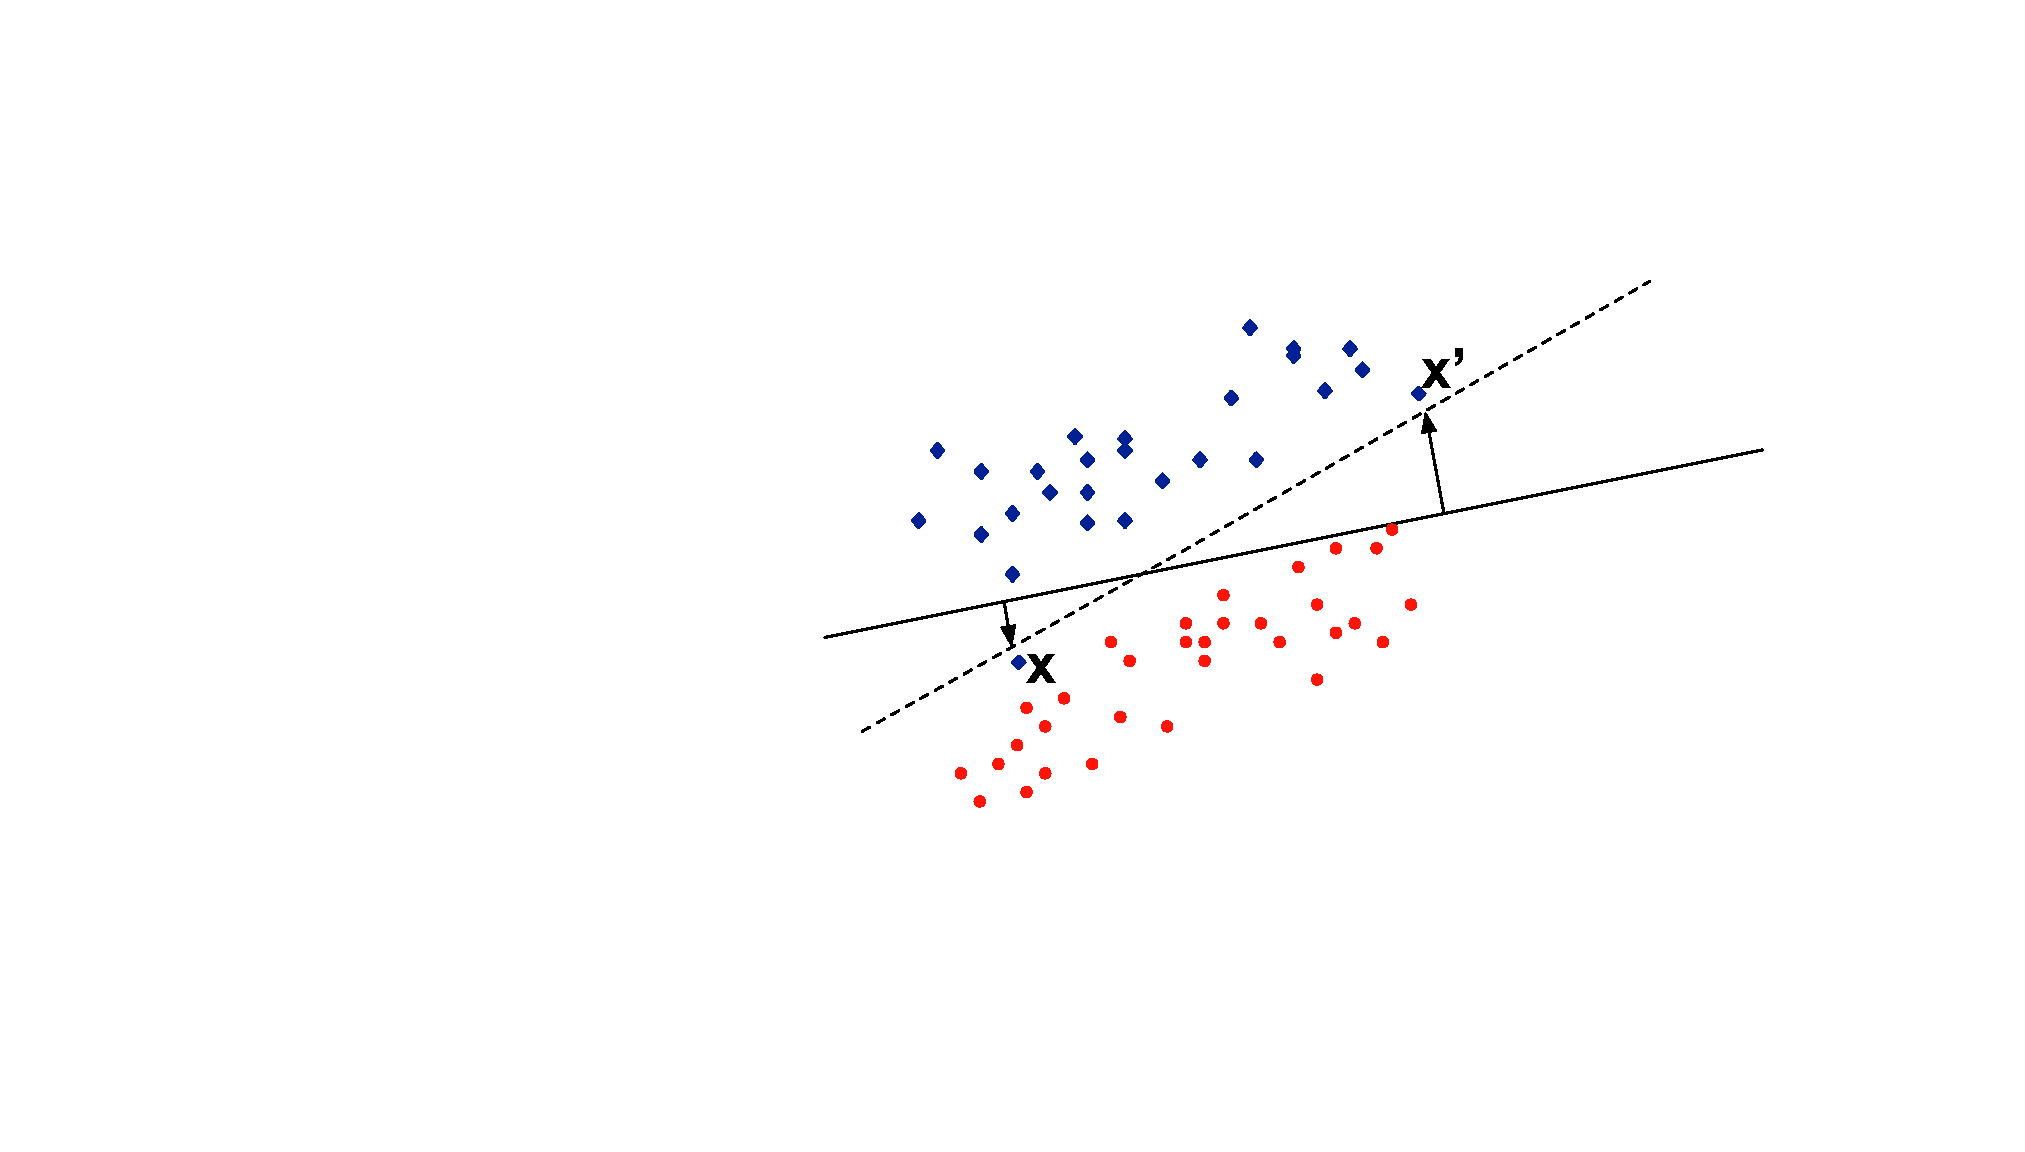
\includegraphics[scale=0.41]{Figures/linear.pdf}
			\label{fig:linear}}
        \hspace{0.2in}
        \subfigure[Neural networks updated by SGD.]{
		\centering
		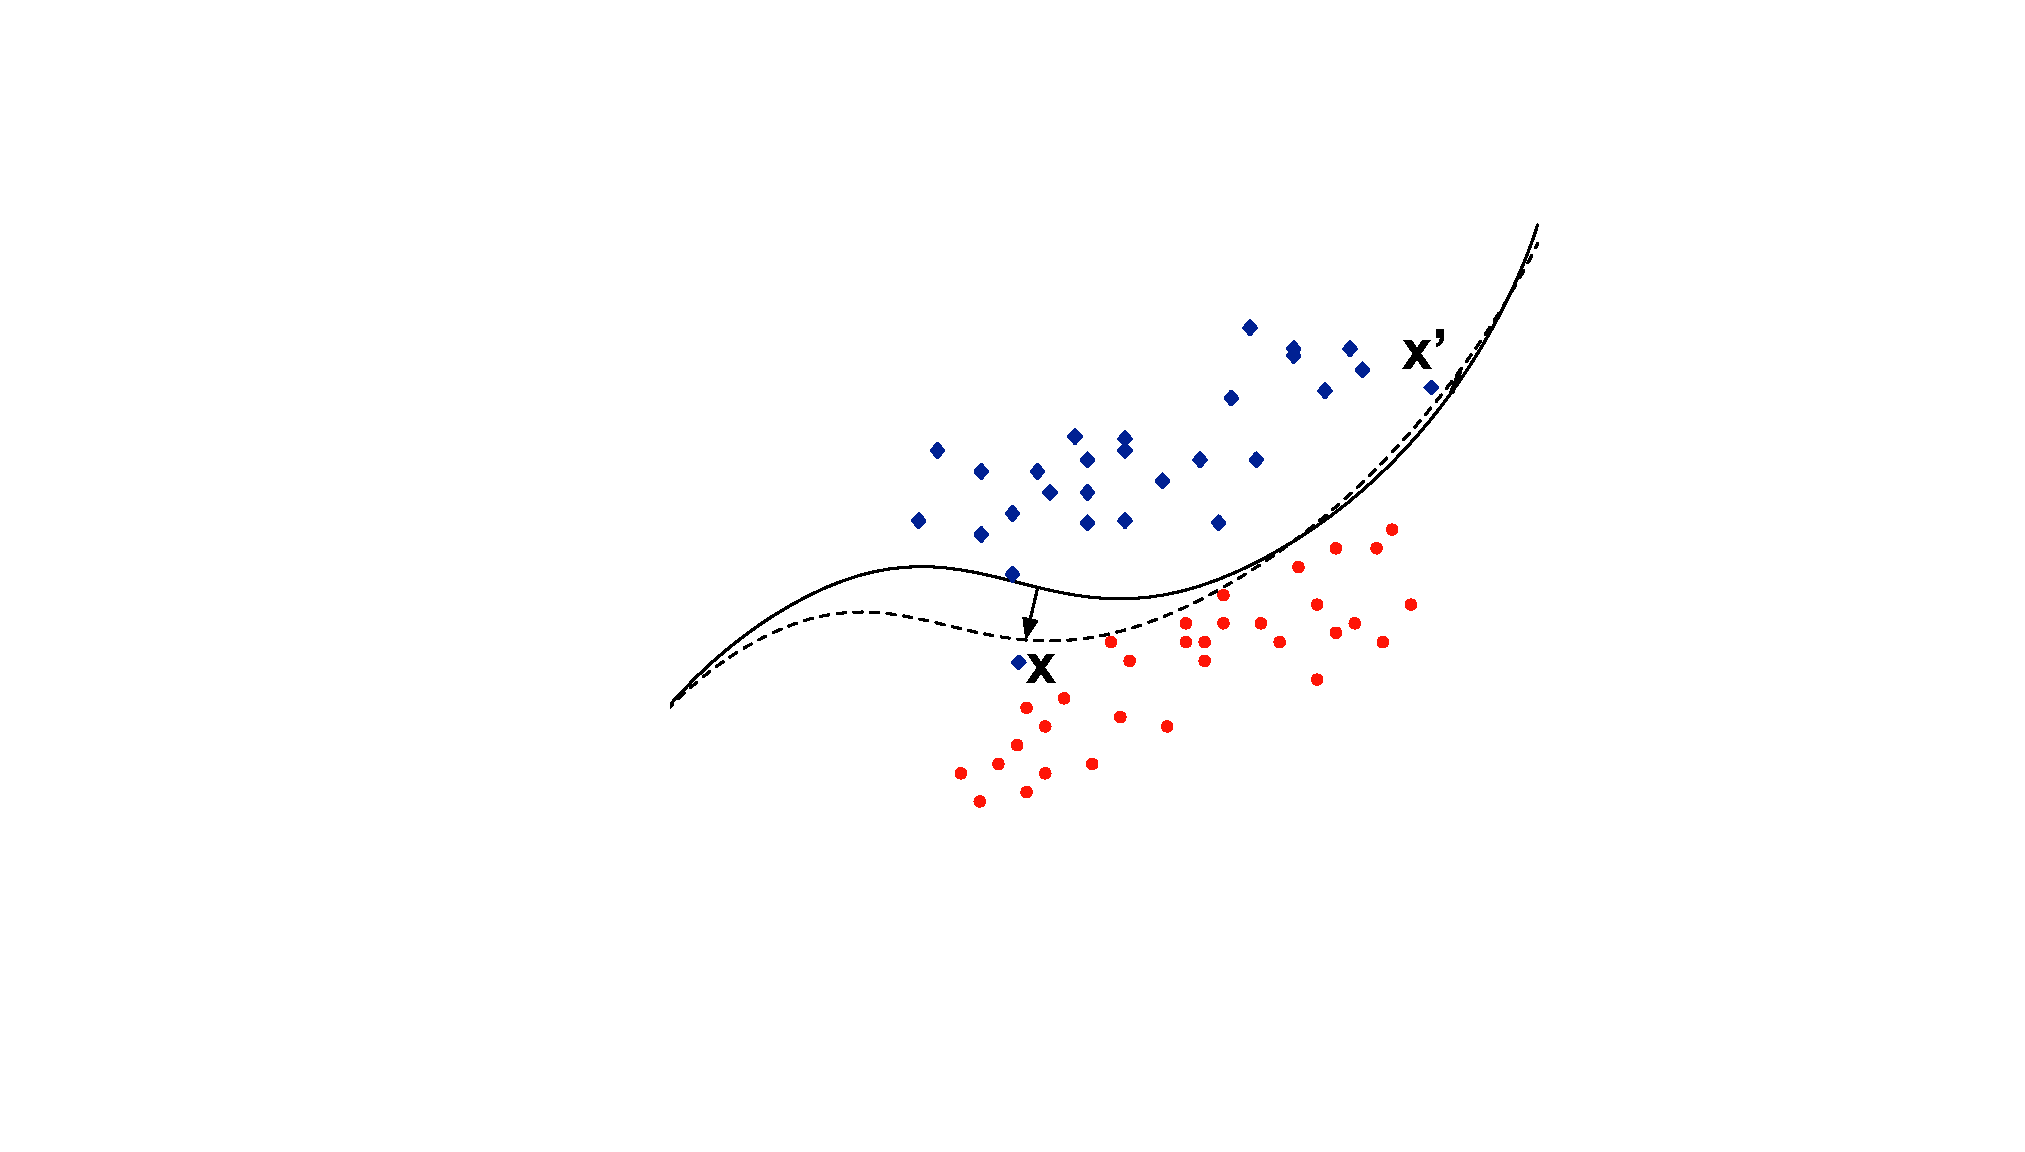
\includegraphics[scale=0.41]{Figures/NNs.pdf}
		\label{fig:NNs}}
        \hspace{0.01in}
        %\subfigure[Each of the two super classes, mammal and vehicle, contains two finer-grained classes. ]{
		%\centering
		%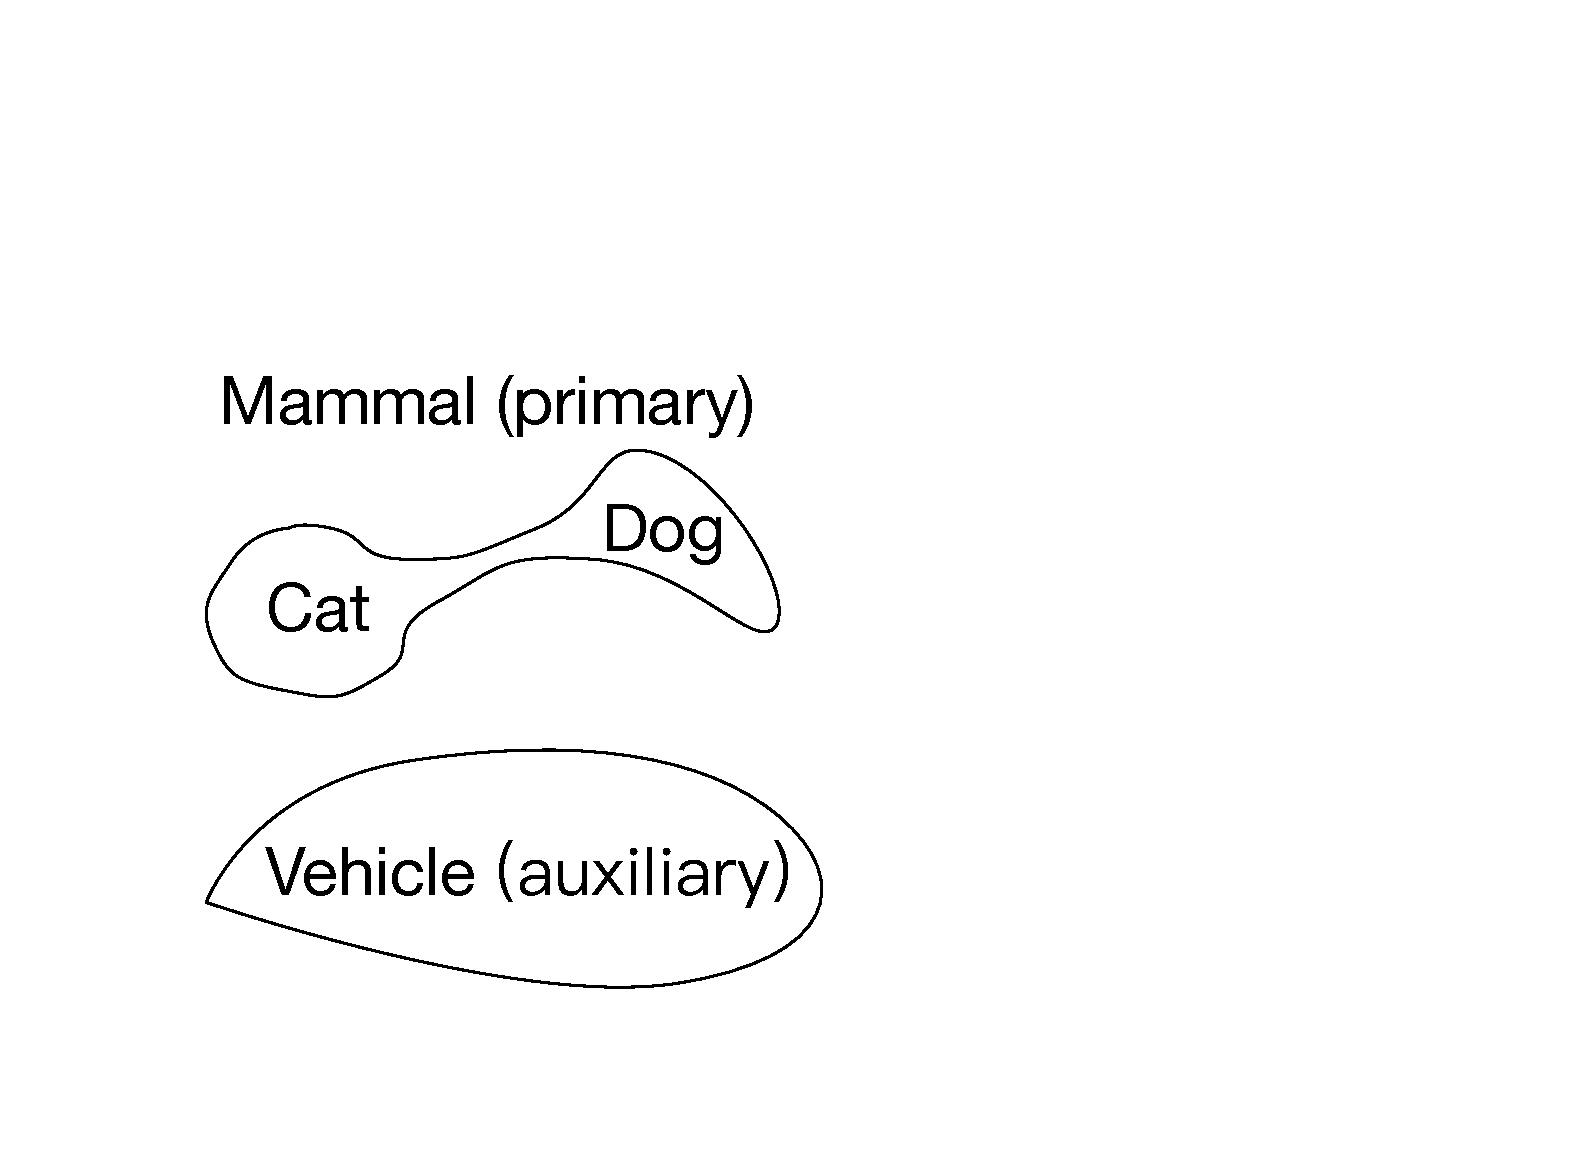
\includegraphics[scale=0.35]{Figures/clusters.pdf}
		%\label{fig:clustering}}
        %\hspace{0.01in}
        \caption{An illustration of linear regression and neural networks updated via SGD. The prediction of $\mbf{x}'$ changes a lot after an SGD update on $\mbf{x}$ in the linear case, though $\mbf{x}'$ is far away from $\mbf{x}$. In contrast, the change in the prediction at $\bx'$ is rather small in the neural networks case.}
		\label{fig:illustration}
\end{figure*}


%%% Local Variables:
%%% mode: latex
%%% TeX-master: "paper"
%%% End:
